\documentclass[12pt,a4paper]{article}
\usepackage[utf8]{inputenc}
\usepackage[portuguese]{babel}
\usepackage[T1]{fontenc}
\usepackage{amsmath}
\usepackage{amsfonts}
\usepackage{amssymb}
\usepackage{graphicx}
\usepackage{fourier}
\usepackage[left=2cm,right=2cm,top=2cm,bottom=2cm]{geometry}
\author{Luiz Guilherme - Professor de Matemática}
\title{Matemática para Concursos Públicos}
\date{Última atualização:  \today} 
\usepackage{tikz}
\usepackage{tcolorbox}
\usepackage{hyperref}
\usepackage{qrcode}
\usepackage{xcolor}
\usepackage{fontawesome}
\usepackage{enumerate}
\usepackage{multicol}

\begin{document}

\newcommand{\quest}[4]{
	\textbf{#1} {\color{red}\faYoutubePlay}\\ % Banca e Concurso
	 {#2}\\ %enunciado
		\begin{minipage}{12cm}
		\begin{enumerate}[a)]
			{#3} %alternativas
		\end{enumerate}
	\end{minipage}
	\qrcode{#4&list=UULFeA_dOOqAA4DB92B_BWDU7Q}} %youtube


\maketitle
\tableofcontents	
\begin{enumerate}

\chapter{Média Aritmética Simples e Ponderada}

\quest{Oficial de Justiça 2023 - VUNESP}{O gráfico apresenta o número de acertos na prova de Língua Portuguesa e de Matemática, aplicada a dois candidatos, A e B, em um concurso interno para promoção de cargo:\\
	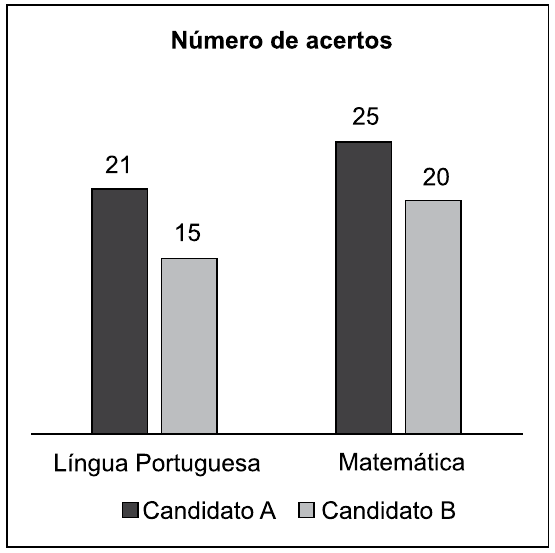
\includegraphics[scale=.5]{fig001.png}\\
Sabendo-se que a prova de Língua Portuguesa tinha 	peso 2 e a de Matemática tinha peso 3 para o cargo em 	concurso, que cada uma das provas tinha 50 questões, 	e que a nota de cada prova é igual ao número de acertos correspondente, é correto afirmar que o número de questões de Matemática que o candidato B deveria ter acertado a mais, para que a média aritmética ponderada das notas das suas provas fosse igual à média aritmética ponderada das notas das provas do candidato A, é igual a}
{\item 9.
\item 20.
\item 10.
\item 29.
\item 27.}
{https://youtu.be/BvsQZctqarQ}

\end{enumerate}



\end{document}